\documentclass[11pt, oneside]{article}   	% use "amsart" instead of "article" for AMSLaTeX format
\usepackage{geometry}                		% See geometry.pdf to learn the layout options. There are lots.
\geometry{letterpaper}                   		% ... or a4paper or a5paper or ... 
%\geometry{landscape}                		% Activate for rotated page geometry
%\usepackage[parfill]{parskip}    		% Activate to begin paragraphs with an empty line rather than an indent
\usepackage{graphicx}				% Use pdf, png, jpg, or eps§ with pdflatex; use eps in DVI mode
								% TeX will automatically convert eps --> pdf in pdflatex		
\usepackage{amssymb}
\usepackage{amsmath}
\usepackage{dcolumn}
\usepackage[table, svgnames, x11names]{xcolor}

\addtolength{\oddsidemargin}{-.875in}
	\addtolength{\evensidemargin}{-.875in}
	\addtolength{\textwidth}{1.75in}

	\addtolength{\topmargin}{-.875in}
	\addtolength{\textheight}{1.75in}



\newcolumntype{d}[1]{D{.}{.}{#1}}

%SetFonts

%SetFonts


\title{Computational modeling}
\author{}
\date{}							% Activate to display a given date or no date

\begin{document}
\maketitle
\section{ISETBio computational model}
\subsection{Overview}
To connect the measured spatial transfer functions (STFs) to the receptive field (RF) organization of the underlying retinal ganglion cells, we employed a computational model which simulates optical, spectral, spatial, and temporal components of the AO stimulation apparatus, as well as the monkey's optics and cone mosaic structure. The model computes a STF, assuming that cone signals are pooled by the center and surround mechanisms of an RGC according to a difference of Gaussians (DoG) spatial profile model. The parameters of the DoG model and therefore, the actual cone pooling weights, are estimating by minimizing the error between the model-- and fluorescence-based-- STFs. A schematic overview of this approach is depicted in Figure \ref{fig:ModelOverview}.

\subsection{AO--based stimulus delivery modeling}
The drifting monochromatic sinusoidal gratings used to measured RGC STFs are modeled as temporal sequences of ISETBio spatial--spectral radiance scenes, where each scene models a different frame of the drifting stimulus.The spectral characteristic, spatial extent and the temporal properties of the AO display subsystem as are all taken into account in generating these scenes. The spectral profile of the monochromatic beam is modeled is Gaussian shaped with a peak at 561 nm and a full-width-half-max bandwidth of 5 nm, and the mean power on the retina is 1.29 $mW / cm^2$. The visual stimulus has a retinal spatial resolution of 1.03 $\mu m$ and its spatial extent is $0.7 \times 0.7$ degrees. All sinusoidal gratings are presented with a nominal contrast of 1.0, and they are drifting at 6.0 $Hz$ with a refresh rate of 25.3 $Hz$ for a duration of 666 msec (4 cycles). 
\begin{table} [h]% put at top of page if possible 
\centering
\begin{tabular}{|r d{3.3}|}
\hline
\rowcolor{LightSlateGray!35!Lavender}  \multicolumn{2}{|l|}{\textbf{visual stimulation modeling}} \\
\hline
\mbox{monochromatic stimulation (peak)} ($nm$) : & 561.0  \\
\mbox{monochromatic stimulation (FWHM)} ($nm$) : & 5.0  \\
\mbox{mean power} ($mW \times cm^{-2}$) : & 1.29  \\
\mbox{retinal pixel size} ($\mu m$) : & 1.03  \\
\mbox{spatial extent} ($degs$) : & \multicolumn{1}{c|}{0.7 $\times$ 0.7}\\
\mbox{contrast} : & 1.0 \\
\mbox{drift rate} ($Hz$) : & 6.0  \\
\mbox{refresh rate} ($Hz$) : & 25.3  \\
\mbox{stimulus duration} (seconds) : & 0.666 \\
\hline
\hline
\rowcolor{LightSlateGray!35!Lavender} \multicolumn{2}{|l|}{\textbf{optics modeling}} \\
\hline
\mbox{pupil diameter} ($mm$) : & 6.7  \\
\mbox{retinal magnification factor} ($\mu m \times deg^{-1}$) : & 199.26 \\
\mbox{AO--residual blur} (diopters) : & \multicolumn{1}{c|}{\mbox{0.067 or variable}}\\

\hline
\hline
\rowcolor{LightSlateGray!35!Lavender} \multicolumn{2}{|l|}{\textbf{cone mosaic modeling}} \\
\hline
\mbox{size} (degs) : & \multicolumn{1}{c|}{1.3 $\times$ 1.3}\\
\mbox{cone density} : & \multicolumn{1}{c|}{\mbox{location dependent, matching AO-measurements}}\\
\mbox{peak cone density} ($10^3 \mbox{cones} \times mm^{-2}$) : & 270.20\\
\mbox{L-cone density} : & \multicolumn{1}{c|}{0.48}\\
\mbox{M-cone density} : & \multicolumn{1}{c|}{0.48}\\
\mbox{S-cone density} : & \multicolumn{1}{c|}{0.04}\\  
\mbox{cone aperture profile} : & \multicolumn{1}{c|}{\mbox{Gaussian}}\\
\mbox{cone characteristic radius, $c_{r_c}$} : & \multicolumn{1}{c|}{0.204 $\times \sqrt{2} \times$
\mbox{inner segment diam}}\\
\mbox{foveal cone characteristic radius (arc.min.)} : & \multicolumn{1}{c|}{0.17}\\
\hline
\hline
\rowcolor{LightSlateGray!35!Lavender} \multicolumn{2}{|l|}{\textbf{RGC modeling (spatial pooling of cone signals)}} \\
\hline
\mbox{peak sensitivity of the center} ($k_c$) : & \mbox{1}\\
\mbox{peak sensitivity of the surround} ($k_s$) : & \multicolumn{1}{c|}{\mbox{variable}}\\
\mbox{characteristic radius of the center} ($r_c$) : & \multicolumn{1}{c|}{$c_{r_c}$ \mbox{(single cone) or variable (multi-cone)}}\\
\mbox{characteristic radius  of the surround} ($r_s$) : & \multicolumn{1}{c|}{\mbox{variable}}\\
\hline
\hline
\end{tabular}
\caption{Parameter values for modeling the AO-based stimulation paradigm, optics, cone mosaic, and RGC spatial pooling.}
\label{table:ModelParameters}
\end{table}

\subsection{Retinal stimulus modeling}
The monkey's optics during AO-based stimulation are modeled as a diffraction-limited optical system model with a 6.7 $mm$ pupil diameter, and a retinal magnification factor of 199.26 $\mu m / \deg$. Residual blur in the AO apparatus, that may be introduced due to a slight defocus of the stimulus with respect to the plane of cone inner segments, is modeled by adjusting the Zernike defocus coefficient.
The amount of residual blur in not known a-priori, and it is estimated from the model as described below. The ISETBio spatial-spectral radiance scenes modeling the AO stimulus are passed via this optical system to generate corresponding spatial-spectral irradiance images, which are processed by the cone mosaic model as described in the next section.

\subsection{Cone mosaic modeling}
An ISETBio model of the monkey's cone mosaic is generated from cone density maps measured during AO imaging, using an iterative approach as described by [Cottaris et al, 2019]. The spatial extent of the model cone mosaic is $1.3 \time 1.3$, with a maximal cone density of 270,200 cones/$mm^2$ with relative densities of 0.48 (L), 0.48 (M), 0.04 (S). Cones are modeled as Gaussian apertures with a characteristic radius equal to $0.204 \times \sqrt{2} \times D$, where $D$ is the inner segment diameter as measured during AO-imaging (Table \ref{table:ModelParameters}). In this cone mosaic model, cone outer-segment lengths, and macular pigment vary with eccentricity, vary with eccentricity as described in [Cottaris et al], and the cone quantal efficiencies are based on the Stockman-Sharpe (2000) normalized absorbance measurements. 

\subsection{Cone excitation response modeling}
To compute a cone's excitation response, the spatial-spectral irradiance impinging on the retina is first spectrally weighted by the product of macular pigment transmittance and by each cone's spectral quantal efficiency, subsequently integrated over wavelength, and spatially integrated over each cone's Gaussian aperture. This excitation response is then integrated over the temporal duration of each stimulus frame (39.5 $msec$), to estimate the expected excitation events count for each cone-$j$, at time $t$, in response to a drifting grating of spatial frequency $\omega$, $E^j(\omega,t)$. In these simulations, we do not include Poisson noise in $E^j(\omega,t)$, nor do we introduce jitter between the cone mosaic and the retinal stimulus due to eye movements.


\subsection{Converting cone excitation responses to cone contrast responses}
Assuming that cones are adapted to the mean background irradiance, the excitations response $E^j(\omega,t)$, is converted to contrast response, $R^j(\omega, t)$, by first subtracting the excitation to the background stimulus, $E^j_o$, and then dividing by it, separately for each cone-$j$, i.e.:
\begin{equation}
R^j(\omega, t) = \frac{E^j(\omega,t) - E^j_o}{E^j_o}
\end{equation}
\noindent where
$E^j_o$ is the excitation of cone-$j$, to the zero contrast (background) stimulus. This operation mimics the photocurrent generation process which converts cone absorption events in the inner segment into ionic currents flowing through the cone outer segment, and which in effect normalizes stimulus-induced excitations responses with respect to the background cone excitation responses.



\subsection{Computing model ganglion cells responses}
Model ganglion cells responses, $\mbox{RGC}(\omega,t)$, are computed from the cone contrast responses assuming linear spatial pooling of cone contrast signals by the antagonistic center and the surround mechanisms, as follows:
\begin{eqnarray}
\mbox{RGC}(\omega,t) & = & \mbox{RGC}_c(\omega,t) - \mbox{RGC}_s(\omega,t) \\
& = & \sum_{j} W_{c}^j  \times R^j(\omega, t) -  \sum_{j} W_{s}^j  \times R^j(\omega, t)
\end{eqnarray}
%
\noindent where, $W_{c}^j, W_{s}^j$, are the factors with which the center and surround mechanisms, respectively, weigh responses $R^j(\omega, t)$, from cone-$j$. There is no temporal filtering, and there is no delay between the center, $\mbox{RGC}_c(\omega,t)$, and surround $\mbox{RGC}_s(\omega,t)$ responses. 

\subsection{Computing model ganglion cell spatial transfer functions}
The spatial transfer function (STF) of a model RGC, $\mbox{STF}^{m}(\omega)$, is computed as: 
\begin{equation}
\mbox{STF}^{m}(\omega) = \mbox{STF}_{c}^{m}(\omega) - \mbox{STF}_{s}^{m}(\omega)
\end{equation}
%
\noindent with
%
$\mbox{STF}_{c}^{m}(\omega)$ and $\mbox{STF}_{s}^{m}(\omega)$ been the STFs of the center and surround mechanisms. These STFs are derived by fitting sinusoidal functions to the center and surround mechanism responses, $\mbox{RGC}_c(\omega,t)$, and $\mbox{RGC}_s(\omega,t)$, respectively, where the sinusoid frequency is set to the temporal frequency of the drifting gratings, and its phase and amplitude are allowed to vary. At each spatial frequency, the amplitude of the best-fit sinusoid is taken as the value of the STF at that spatial frequency. Formulating $\mbox{STF}^{m}$ as the difference of the center and the surround STFs, enables the model STF to achieve negative values, which are some times encountered in the measured fluorescence-based STF responses, $\mbox{STF}^{\Delta F / F}(\omega)$, at the lowest spatial frequencies. An alternative, would be to fit sinusoidal functions to the composite response, $\mbox{RGC}(\omega,t)$, but in that case the derived STFs cannot have negative values, and the fits to certain $\mbox{STF}^{\Delta F / F}(\omega)$ measurements become sub-optimal.

\subsection{Estimating model RGC cone pooling weights from fluorescence-based STF measurements}
%
The weights with which the center and surround mechanisms of a model RGC, are pooling signals from a cone-$j$ are derived assuming a Gaussian pooling profiles,
\begin{eqnarray}
W_c^j  & = & \begin{cases}
    \exp \left [ -\left( d_{j}/r_c \right) ^2 \right ], & \text{for the multi-cone RF center model}.\\
   1, & \text{for the single-cone RF center model}.
   \end{cases} \\
W_s^j &= &k_s \times \exp \left [ -\left( d_{j}/r_s \right) ^2 \right ]
\end{eqnarray}
\noindent where $d_j$ is the distance between cone-$j$ and the spatial position of the center mechanism of the model RGC (which is the spatial position of the cone driving the center mechanism). The parameters $k_s$, $r_c$, and $r_s$, which represent the surround peak sensitivity and the center and surround characteristic radii, respectively, of the Difference of Gaussians (DoG) RF model, are determined by minimizing the weighted error between the model STF, $\mbox{STF}^{m}(\omega)$, and the measured STF, $\mbox{STF}^{\Delta F / F}(\omega)$, accumulated over all spatial frequencies, $\omega$:

\begin{equation}
\mbox{RMSE} = \displaystyle \sum_{\omega} \frac{1}{\epsilon({\omega})} \times {\left [  \mbox{STF}^{m}(\omega)  - \mbox{STF}^{\Delta F / F}(\omega) \right ] }^2
\end{equation}
where $\epsilon({\omega})$ is the standard error of the mean of the $\mbox{STF}^{\Delta F / F}(\omega)$ measurement. To minimize the chance of getting stuck to local minima of the error function, we employ a multi-start minimizer which is ran 256 times, keeping the results from the run which results in the minimum RMSE.


\subsection{Model validation \& model selection}
To validate the extracted model RGC parameters ($k_s$, $r_c$ and $r_s$), we employ a cross-validation approach, in which we train the model by minimizing the error between $\mbox{STF}^{m}_{s_{train}}$ and the fluorescence-based STF, $\mbox{STF}^{\Delta F / F}_{s_{train}}$, measured at one recording session, $s_{train}$, while assessing model performance by computing the error between $\mbox{STF}^{m}_{s_{train}}$ and $\mbox{STF}^{\Delta F / F}_{s_{test}}$, with $s_{test} \ne  s_{train}$. In this, cross-session comparison, we allow for an arbitrary scaling of $\mbox{STF}^{m}_{s_{train}}$ by a factor $\gamma$, which is selected so as to minimize the cross-validated error between the model STF computed using data from the $s_{train}$ session, and the fluorescence--based STF measured at the $s_{test}$ session: 
%
\begin{equation}
\mbox{cv-RMSE}^{s_{test}}_{s_{train}} = \min_{\gamma} \left( \sum_{\omega} \left [  \frac{\gamma \times \mbox{STF}^{m}_{s_{train}}(\omega) - \mbox{STF}^{\Delta F / F}_{s_{test}}(\omega)}{IQR} \right ] ^2 \right)
\end{equation}
%
\noindent
where $IQR$ is the interquartile range of $\mbox{STF}^{\Delta F / F}_{s_{test}}(\omega)$. Division with the $IQR$ of the measured data standardizes the error with respect to the scale of the data, which would be different across different $s_{test}$ sessions.

Averaging $\mbox{cv-RMSE}^{s_{test}}_{s_{train}}$ over all test sessions, we obtain the overall cross-validated RMSE for each training session, $\mbox{cv-RMSE}_{s_{train}}$, and repeating this for all training sessions, we find the training session, $s_{train}^{best}$, with the minimal cross-validation error, $\mbox{cv-RMSE}_{s_{train}^{best}}$. The model computed at the $s_{train}^{best}$ session is considered to have the best generalizing performance.

Finally, since the receptive field location of the recorded RGCs is only known approximately to lie within the central 40 $\mu m$, we compute $\mbox{cv-RMSE}^{CV}_{s_{train}^{best}}$ repeatedly, each time assuming that the model RGC receives its center-driving signal from cones in different parts of the central 40 $\mu m$ of the model cone mosaic. Searching for the minimum $\mbox{RMSE}^{CV}_{s_{train}^{best}}$ over all examined center-cone positions, we determine the best-generalizing model with the lowest cross-validation error amongst all examined RF center positions.

\subsection{Assessing performance across different models}
This cross-validation model selection approach can also be used to compare performance in models with different number of parameters. Without cross-validation, model with more parameters are more likely to overfit the data and have seemingly better performance. With cross-validation, overfitting becomes less likely, and selecting the best model becomes more meaningful. 

We examined how different models can explain the measured STF responses (Table \ref{table:ModelAssessment}).

\begin{table}[h]
\centering
\begin{tabular}{|l | l  l |l |}
\hline
\rowcolor{LightSlateGray!35!Lavender}  \multicolumn{1}{|l|}{\textbf{model description}} & \textbf{variable params} & \textbf{fixed params} & \textbf{result} \\
\hline
\hline
single cone center, zero residual defocus        & $k_c, k_s, r_s$                 &  $r_c = c_{r_c}, z_{d} = 0.000D$ & worse cv-RMSE \\
single cone center, single residual defocus        & $k_c, k_s, r_s$                 &  $r_c = c_{r_c}, z_{d} = 0.067D$ & pending \\
single cone center, variable residual defocus      & $k_c, k_s, r_s, z_{d}$ & $r_c = c_{r_c}$ & pending \\
multiple cone center, zero residual defocus        & $k_c, k_s, r_c, r_s$                 &  $r_c = c_{r_c}, z_{d} = 0.000D$ & pending \\
multiple cone center, variable residual defocus    & $k_c, k_s, r_c, r_s, z_{d}$ & -- &  pending \\
\hline
\end{tabular}
\caption{Examined models}
\label{table:ModelAssessment}
\end{table}

\section{Results}

\begin{figure}[htbp] %  figure placement: here, top, bottom, or page
   \centering
   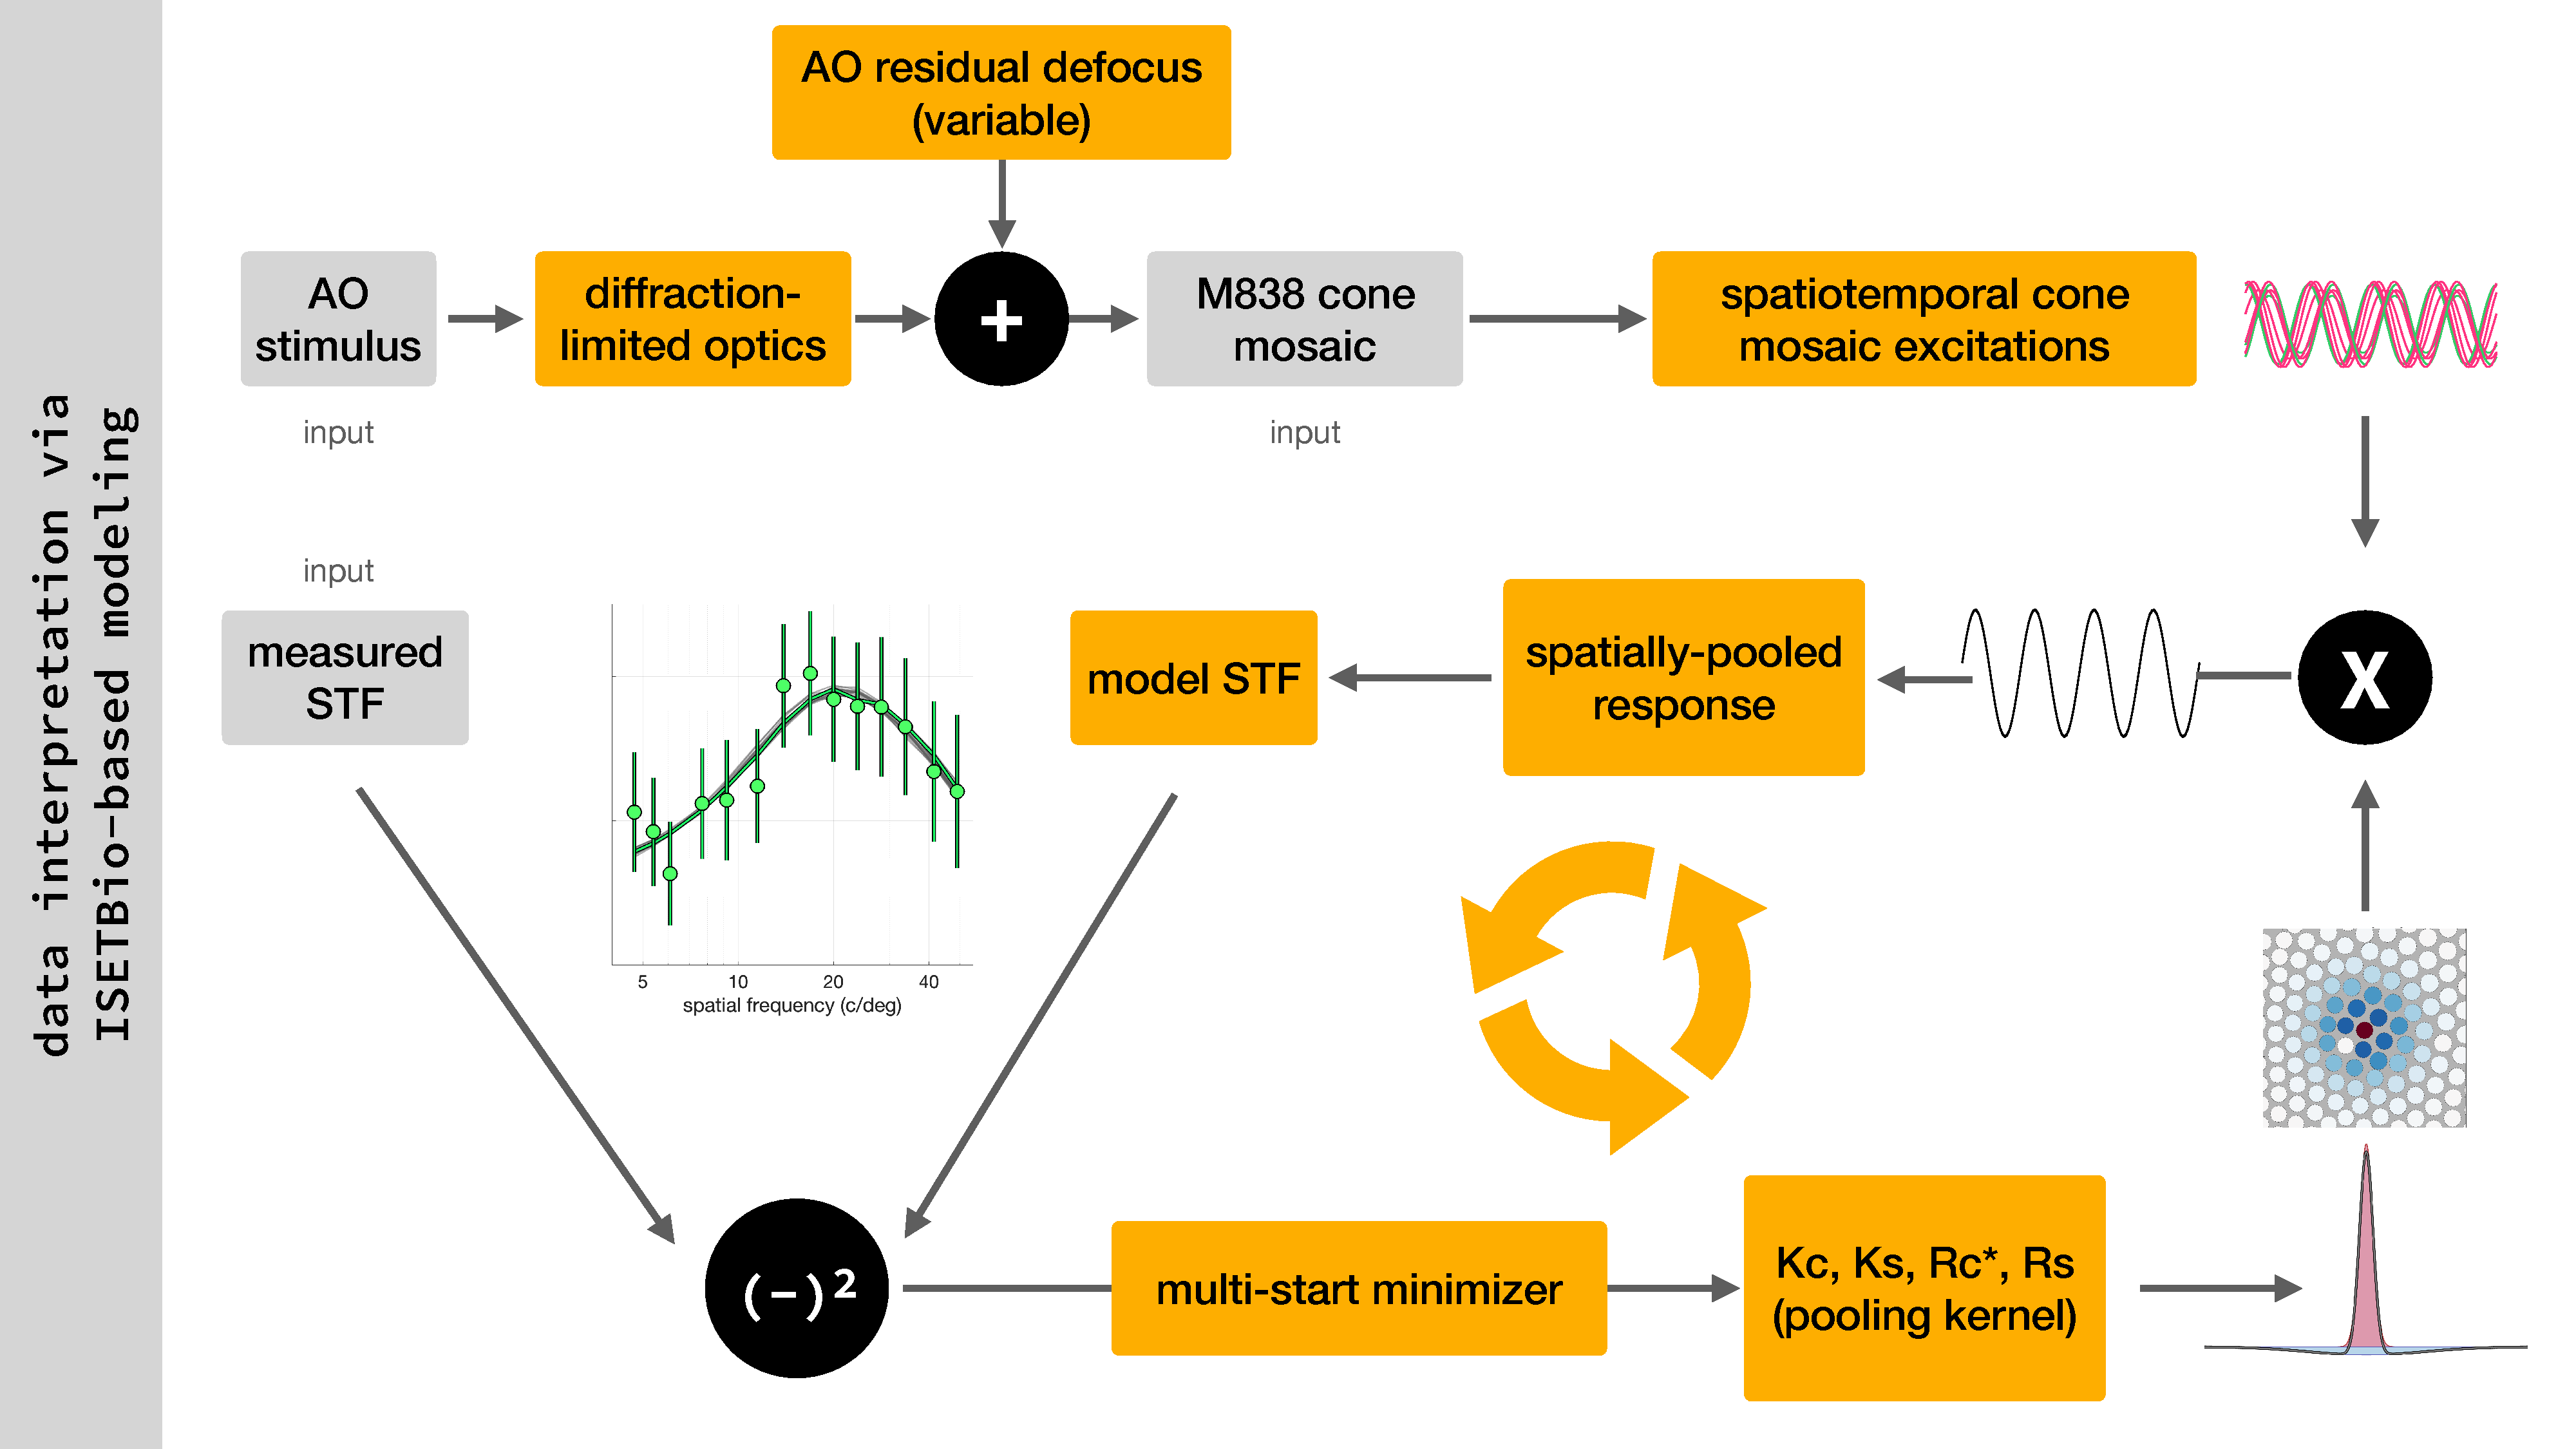
\includegraphics[width=7in]{Figures/ModelOverview.pdf} 
   \caption{Schematic overview of the ISETBio computational model.}
   \label{fig:ModelOverview}
\end{figure}



\end{document}  